\chapter{Development of new stages}
New \acrshort{fapec} stages must be well documented, efficient and easy to maintain. In order to achieve this, all stages are subject to some general requirements and must be evaluated. In this chapter we will first list the general requirements for new stages. Then, we will present four metrics to evaluate each stage.

\section{Requirements for \acrshort{fapec} stages} \label{sec:fapec_reqs}
In this section we will list the general requirements that all \acrshort{fapec} stages developed by DAPCOM must fulfill. Besides these, other specific requirements for each stage may be defined.

\subsubsection{Requirements}
\begin{enumerate}
	\item The stage must be implemented in C. \label{req:c}
	\item The software shall be provided as a library and as a stand-alone binary. \label{req:lib_bin}
	\item The stage must be able to work with data chunks. \label{req:chunks}
	\item The stage must support lossless and lossy compression.
	\item Data must not be lost even if the input is corrupted (i.e. delta fallback).
	\item Compression ratio shall be better than Gzip's.
	\item Compression speed shall be better than Gzip's.
	\item The software shall be tested with a representative dataset.
	\item The design and implementation must be documented.
\end{enumerate}

\subsubsection{Specifications}
The following specifications shall be fulfilled with an Intel Core i7-10710U \acrshort{cpu}.

\begin{enumerate}
	\item The occupied memory with one thread shall not exceed 64 MB.
	\item \acrshort{fapec} data chunks shall have a size between 128 kB and 4 MB.
	\item Decompression time can't be higher than a 110\% of the compression time.
	\item At least a 10\% of the source code lines must be comments.
	\item McCabe complexity \parencite{mccabe} shall be below 50.
\end{enumerate}

\section{Evaluation of stages}
The aim of this section is to present the metrics used in the following chapters to evaluate the developed preprocessing stages. The proposed indexes may be classified in two groups: information metrics and performance metrics.

\subsection{Information metrics}
This subset of metrics is purely focused on evaluating how better data are after the decorrelation stage. Our first approach is to plot a \textbf{histogram} of the original samples together with a histogram of the prediction errors (i.e. the values that will be sent to the \acrshort{fapec} entropy coder). For a better visualization, the bin width is calculated from the number of samples and it is the same for both histograms. Besides, the prediction errors histogram is also doted with three vertical lines at percentiles 5, 50 and 95 in order to clearly show the range where 90\% of data is contained.

Making use of the histograms, the \textbf{cumulative histograms} of the original samples and the prediction errors are calculated and plotted together. Although this graphics are just the integral of the histograms described above, they provide a clear way to see samples concentration in intervals.

\begin{figure}[h!]
	\centering
	\begin{subfigure}{0.5\textwidth}
		\centering
		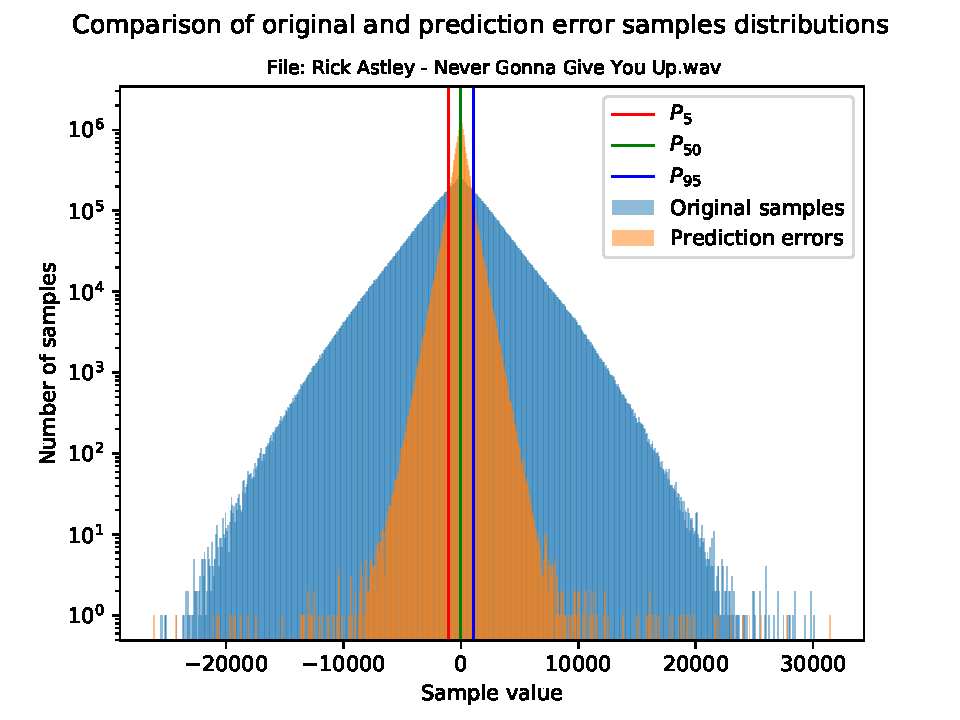
\includegraphics[width=\linewidth]{images/Rick Astley - Never Gonna Give You Up.wav_hist.pdf}
		\caption{Histogram of an audio file.}
		\label{fig:hist_example}
	\end{subfigure}%
	\begin{subfigure}{0.5\textwidth}
		\centering
		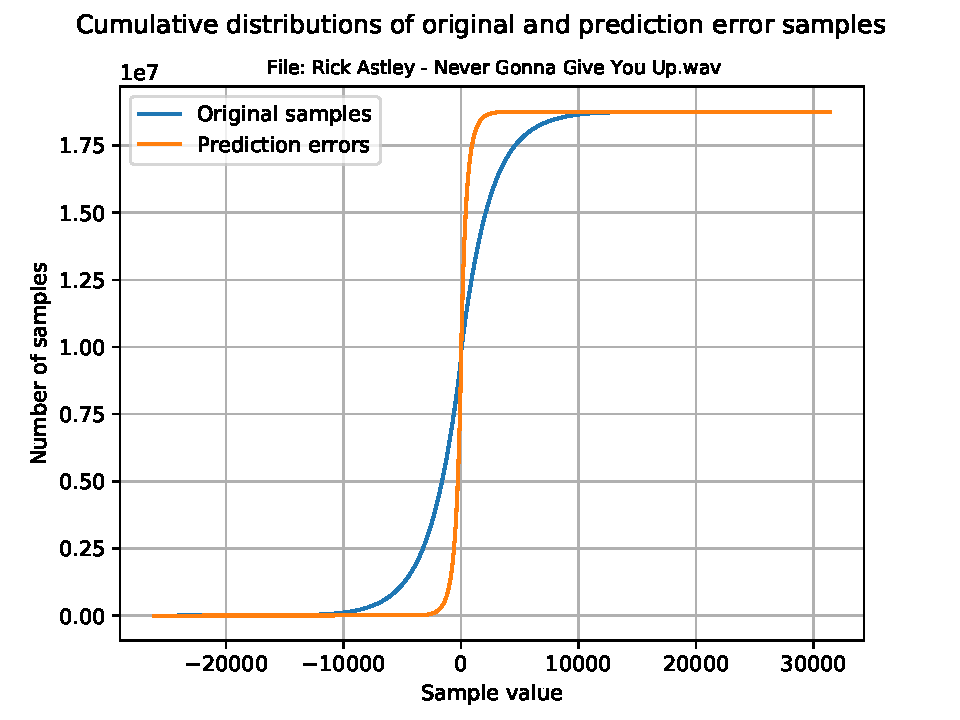
\includegraphics[width=\linewidth]{images/Rick Astley - Never Gonna Give You Up.wav_hist_cum.pdf}
		\caption{Cumulative histogram of an audio file.}
		\label{fig:sub2}
	\end{subfigure}
	\caption{Histogram and cumulative histogram of a file compressed with Wave.}
	\label{fig:test}
\end{figure}

At the beginning of this thesis no more information metrics were planned, but we realized that these two are subject to data scaling. That is, with a simple division the metric can be adulterated. In order to deal with it, we also propose to use \textbf{negentropy} (see section \ref{sec:negentropy}) to measure how compressible the prediction errors are compared with the original samples. There are two main reasons behind choosing negentropy: the first is that it is invariant to linear maps, and the second is that it is a measure of non-Gaussianity. The first property solves the problem of data scaling, and the second one offers a way of knowing if the stage has improved data distribution (i.e. negentropy is higher).

Although negentropy is a highly suitable metric for our purposes, it has an important drawback: its calculation is computationally very complex. Moreover, estimating it from data requires estimating the probability density function of the samples to later plug it into the definition of differential entropy and finally subtracting it to the Gaussian entropy for the same variance. However, negentropy can be approximated with the following expression \parencite{HYVARINEN2000411}:
\begin{equation}
J(X) \propto \left[E[G(X)] - E[G(V)]\right]^2
\end{equation}
where $X$ is a random variable with $\mu = 0$ and $\sigma = 1$, $V \sim N(0,1)$ and $G(u)$ is a non-quadratic function. In our case, $X$ and $V$ will be data arrays and
\begin{equation}
G(u) = \ln \cosh u
\end{equation}

\subsection{Performance metrics}
We are interested in comparing the whole compression process: from opening the original file to writing the encoded one. In other words, we want to evaluate the performance of the decorrelation stage plus the entropy coder compared with other compressors.

In this thesis we propose a new metric based on Euclidean distance that takes into account the (normalized) process time and the (inverse) compression ratio. Mainly, given an input file, it consists in computing a dot in $\mathbb{R}^2$ where the first coordinate is the normalized process time and the second is the inverse of the compression ratio. Then, the Euclidean distance to the origin is computed for every algorithm and the one with the smallest distance is assumed to be the best. Formally, the coordinates for each compressor are given by
\begin{equation} \label{eq:dot_comp}
\mathbf{a} = \left(t, \frac{s_c}{s_o}\right)
\end{equation}

and the metric is
\begin{equation} \label{eq:metric_gamma}
\gamma = \left\Vert \mathbf{a} \right\Vert ^2 = t^2 + \left(\frac{s_c}{s_o}\right)^2
\end{equation}

where $t$ is the process time normalized by 1 second, $s_c$ the compressed file size in bytes and $s_o$ the original file size also in bytes.

In order to reliably calculate the compression time, each compressor is run as a child-process on a Python script. Then, time is taken before spawning the child-process and again after it exits. Subtracting the end time to the start time gives the process time which, divided by 1 second, is used in equations \ref{eq:dot_comp} and \ref{eq:metric_gamma}.

Finally, we want to point out that in the following chapters the metric $\gamma$ will be given together with a plot including the dot $\mathbf{a}$ for several input files and compressors.
